%===============================================================================
%	REPORT TEMPLATE
%===============================================================================

\documentclass[a4paper, 11pt, fleqn, oneside]{book}
%\documentclass[a4paper, 11pt, fleqn, twoside]{book}

%-------------------------------------------------------------------------------
%	METADATA AND SETTINGS
%-------------------------------------------------------------------------------

%===============================================================================
%	SETTINGS
%===============================================================================

%-------------------------------------------------------------------------------
% PACKAGES IMPORT AND CONFIGURATIONS
%-------------------------------------------------------------------------------

\usepackage[T1]{fontenc}
\usepackage[utf8]{inputenc}
\usepackage[english, french]{babel}
\usepackage{courier} % To display code in a descent font
\usepackage[top=37mm, bottom=42mm, left=36mm, right=29mm]{geometry}
\usepackage{fancyhdr}
\usepackage{listings}
\usepackage{graphicx} % Required to insert images
\usepackage{titlesec}
\usepackage{hyperref} % Required for cross-references
\usepackage[export]{adjustbox} % Required to add frame around figures
\usepackage{float} % To put figure etc where you want
\usepackage[usenames,dvipsnames]{color} % Required for custom colors
\usepackage[table]{xcolor} 
\usepackage{microtype} % Typographic improvements
\usepackage{setspace} % increase interline spacing slightly
\usepackage{subfig}
\usepackage{booktabs}
\usepackage{lipsum} % To easily add lorem ipsum
\usepackage{url}
\usepackage{amsmath}
\usepackage[final]{pdfpages}
\usepackage[toc, page]{appendix}


%-------------------------------------------------------------------------------
% PACKAGE OPTIONS
%-------------------------------------------------------------------------------

% color
%-------------------------------------------------------------------------------
\definecolor{gray75}{gray}{0.75}
\definecolor{gray20}{gray}{0.8}
\definecolor{light-gray}{gray}{0.50}
\definecolor{very-light-gray}{gray}{0.9}
\definecolor{MyDarkGreen}{rgb}{0.0,0.4,0.0} % This is the color used for comments

% Listings
%-------------------------------------------------------------------------------

% Language loading
% --------------------------------
\lstloadlanguages{Java} % Load Java syntax for listings, for a list of other languages supported see: ftp://ftp.tex.ac.uk/tex-archive/macros/latex/contrib/listings/listings.pdf

% Language styling
% --------------------------------
\lstset{
        breaklines=true,
        postbreak=\raisebox{0ex}[0ex][0ex]{\ensuremath{\color{red}\hookrightarrow\space}},
        language=Java, % Use Java
        frame=single, % Single frame around code
        basicstyle=\usefont{T1}{pcr}{m}{s}\footnotesize, % Use small true type font
        keywordstyle=[1]\usefont{T1}{pcr}{m}{s}\color{Purple}\footnotesize\bf, % Perl functions bold and blue
        keywordstyle=[2]\color{Blue}, % Perl function arguments purple
        keywordstyle=[3]\color{Blue}\underbar, % Custom functions underlined and blue
        identifierstyle=, % Nothing special about identifiers
        commentstyle=\usefont{T1}{pcr}{m}{s}\color{MyDarkGreen}\footnotesize, % Comments small dark green courier font
        stringstyle=\color{Blue}, % Strings are purple
        showstringspaces=false, % Don't put marks in string spaces
        tabsize=4, % 4 spaces per tab
        %
        % Put standard Perl functions not included in the default language here
        morekeywords={rand},
        %
        % Put Perl function parameters here
        morekeywords=[2]{on, off, interp},
        %
        % Put user defined functions here
        morekeywords=[3]{test},
        %
        morecomment=[l][\color{Blue}]{...}, % Line continuation (...) like blue comment
        numbers=left, % Line numbers on left
        numberstyle=\tiny\color{light-gray},  % the style that is used for the line-numbers
        numbersep=5pt,                  % how far the line-numbers are from the code
        firstnumber=1, % Line numbers start with line 1
        %stepnumber=5 % Line numbers go in steps of 5
}

% graphix
%-------------------------------------------------------------------------------
\graphicspath{{img/}}

% setspace
%-------------------------------------------------------------------------------
\setstretch{1.1}

\makeatletter
\setlength{\@fptop}{0pt}  % for aligning all floating figures/tables etc. to the top margin
\makeatother


% Fancyhdr
%-------------------------------------------------------------------------------
\renewcommand{\sectionmark}[1]{\markright{\thesection\ #1}}

\pagestyle{fancy}
  \fancyhf{}
  \renewcommand{\headrulewidth}{0.4pt}
  \renewcommand{\footrulewidth}{0pt}
  \fancyhead[OR]{\bfseries \nouppercase{\rightmark}}
  \fancyhead[EL]{\bfseries \nouppercase{\leftmark}}
  \fancyfoot[EL,OR]{\thepage}

\fancypagestyle{plain}{
  \fancyhf{}
  \renewcommand{\headrulewidth}{0pt}
  \renewcommand{\footrulewidth}{0pt}
  \fancyfoot[EL,OR]{\thepage}}

\fancypagestyle{addpagenumbersforpdfimports}{
  \fancyhead{}
  \renewcommand{\headrulewidth}{0pt}
  \fancyfoot{}
  \fancyfoot[RO,LE]{\thepage}
}


% Hyperref
%-------------------------------------------------------------------------------

\hypersetup{pdfborder={0 0 0},
	colorlinks=true,
	linkcolor=black,
	citecolor=black,
	urlcolor=black}
\urlstyle{same}

\makeatletter
\def\cleardoublepage{\clearpage\if@twoside \ifodd\c@page\else
    \hbox{}
    \thispagestyle{empty}
    \newpage
    \if@twocolumn\hbox{}\newpage\fi\fi\fi}
\makeatother \clearpage{\pagestyle{plain}\cleardoublepage}


% Titlesec
%-------------------------------------------------------------------------------

\newcommand{\hsp}{\hspace{20pt}}

% Change chapter title style
% --------------------------------
\titleformat{\chapter}[block]
{\Huge\bfseries}
{\thechapter\hsp\textcolor{gray75}{|}\hsp}
{0pt}
{\Huge\bfseries}

\titlespacing*{\chapter}
{0pt}
{-50pt}
{20pt}

% Change section title style
% --------------------------------
\titleformat{\section}[block]
{\Large\bfseries}
{\thesection}
{0.5em}
{}
 
\titlespacing*{\section}
{0em}
{1.5ex plus .1ex minus .2ex}
{0.8em}

% Change subsection title style
% --------------------------------
\titleformat{\subsection}[block]
{\large\bfseries}
{\thesubsection}
{0.5em}
{}
 
\titlespacing*{\subsection}
{0em}
{1.5ex plus .1ex minus .2ex}
{0.3em}

% Change subsubsection title style
% --------------------------------
\titleformat{\subsubsection}[block]
{\normalsize\bfseries}
{\thesubsubsection}
{0.5em}
{}
 
\titlespacing*{\subsubsection}
{0em}
{1.5ex plus .1ex minus .2ex}
{0em}

% Amsmath
%-------------------------------------------------------------------------------
%Fix the problem with delimiter size caused by fourier and amsmath packages.
\makeatletter
\def\resetMathstrut@{%
  \setbox\z@\hbox{%
    \mathchardef\@tempa\mathcode`\(\relax
      \def\@tempb##1"##2##3{\the\textfont"##3\char"}%
      \expandafter\@tempb\meaning\@tempa \relax
  }%
  \ht\Mathstrutbox@1.2\ht\z@ \dp\Mathstrutbox@1.2\dp\z@
}
\makeatother


\usepackage[semester]{metadata}

\university{Haute école spécialisée de Suisse occidentale}
\study{Technologies de l'information et de la communication}
\faculty{MSE - Software Engineering}
\course{Data Management}
\title{Lab 01 - Création et exploration d'un cube OLAP}
\location{Lausanne}

% Students
% --------------------------------
\newcommand{\mAuthors}{
	Robin Chappatte\\
	Frédéric Montet\\
	Brian Nydegger
}

% Supervisors (Professors)
% --------------------------------
\newcommand{\mSupervisors}{
	Dr. Laura Elena Raileanu\\
	Fabien Dutoit
}

%-------------------------------------------------------------------------------
%	DOCUMENT
%-------------------------------------------------------------------------------


%	HEAD: Book-Begin
%-------------------------------------------------------------------------------
\begin{document}

\frontmatter
\begin{titlepage}
    \newgeometry{top=25mm, bottom=25mm, left=36mm, right=29mm}
    \begin{flushleft}

        \begin{minipage}[c][1.5cm][t]{0.4\textwidth}
            \begin{flushleft}
                \vspace{0.1cm}
                
\includegraphics[width=200pt]{img/mse.eps}
            \end{flushleft}
        \end{minipage}
        \hfill
        \begin{minipage}[c][1.5cm][t]{0.4\textwidth}
            \begin{flushright}
                
\includegraphics[width=100pt]{img/hesso.eps}
            \end{flushright}
        \end{minipage}

        \makeatletter

        \vspace{3cm}

        {\huge \bfseries \@course \par}
        {\Large \@title \par}

        \vspace{1cm}

        \mAuthors

        \vspace{0.6cm}
        
        Rendu le \today \\
        à \@location

        \vspace*{\fill}

        \begin{minipage}[t]{0.49\textwidth}
            \begin{flushleft}
                \textbf{Professeurs :} \\
                \mSupervisors\\
            \end{flushleft}
         \end{minipage}

        \vspace{2cm}
        \makeatother

        \end{flushleft}
        \begin{center}
             {HES-SO\thinspace//\thinspace Master, Lausanne, \the\year}\\
        \end{center}
    \restoregeometry
\end{titlepage}
\setcounter{page}{0}

\tableofcontents
\clearpage

% % space before each new paragraph according to the template guidelines.
% %(needs to be after titlepage and frontmatter to keep the table of contents lists short)
\setlength{\parskip}{1em}


%	MAIN: The chapters of the report
%-------------------------------------------------------------------------------
\mainmatter
\chapter*{Introduction}
\addcontentsline{toc}{chapter}{Introduction}

%TODO


\chapter{Installation}

L'infrastructure nécessaire pour l'utilisation d'un cube OLAP consiste en l'installation de 2 serveurs:

\begin{enumerate}
	\item MySQL
	\item icCube
\end{enumerate}

\section{MySQL}

L'installation du serveur MySQL a été simplifiée en utilisant la plateforme de développement web Wamp, réspectivement Mamp pour OSX ou encore Xamp pour Linux.
Ainsi, la configuration de ces outils est déjà faite et, de plus, des outils d'administration de base de donnée comme PhpMyAdmin y sont disponible.

\section{icCube}

L'installation du serveur OLAP icCube se fait de la même manière qu'une application commerciale grand publique, il suffit de suivre l'assistant d'installation. Sa seule dépendance est Java 1.8. 

Une fois l'installation faite, le serveur OLAP est disponible à l'adresse \texttt{\url{http://localhost:8282/icCube/icCube_en.html}}.

\chapter{Configuration}

Les étapes de configuration de MySQL et icCube converge vers l'objectif commun d'avoir un cube OLAP sur lequel il est possible d'effectuer des requètes multi-dimensionnelles. 

\section{Importation des données dans MySQL}

Après avor créé un nouvel utilisateur MySQL, nous avons importé les données du dump \texttt{aventure2014.sql.gz}.

Les données importées proviennent d'une base de données fournie par Microsoft. Il s'agit de 120'000 ventes d'articles de vélo, par internet et en magasin dans plusieurs pays. Le diagramme ER\footnote{Entity-Relationship} est visible sur la figure \autoref{img:er-diagramm}. 

\begin{figure}[H]
    \centering
    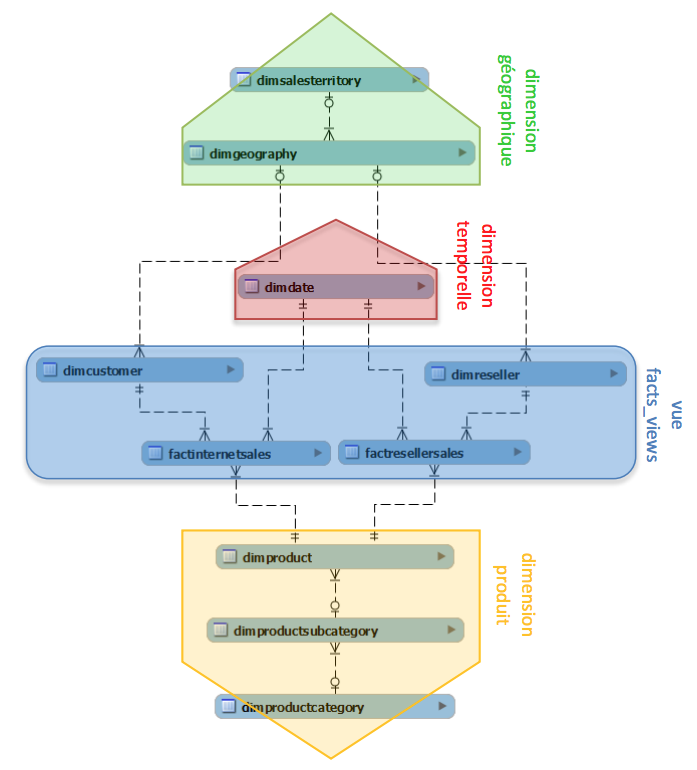
\includegraphics[width=0.7\linewidth, fbox]{img/er_diagramm.png}
    \caption{Entity Relationship diagramm}
    \label{img:er-diagramm}
\end{figure}

\subsection{Création d'une vue}

Pour préparer les différentes dimensions que nous souhaitons avoir avec notre cube OLAP, une vue supplémentaire est nécessaire. Il s'agit de la \texttt{product\_view} qui a été créée avec la requète \autoref{lst:sqlProductView}

\begin{figure}[H]
\centering
\begin{lstlisting}	
CREATE VIEW product_views AS 
SELECT dp.ProductKey, dp.EnglishProductName, dp.ProductSubcategoryKey, dps.EnglishProductSubcategoryName, dps.ProductCategoryKey, dpc.EnglishProductCategoryName 
FROM dimproduct AS dp 
LEFT JOIN dimproductsubcategory AS dps 
ON dps.ProductSubcategoryKey = dp.ProductSubcategoryKey 
LEFT JOIN dimproductcategory AS dpc 
ON dpc.ProductCategoryKey = dps.ProductCategoryKey
\end{lstlisting}
\caption{Requête SQL pour la création de la vue des produits}
\label{lst:sqlProductView}
\end{figure}


\section{Configuration d'icCube}

\subsection{Dimension temporelle}

% Pour la dimension temporelle, vous créerez 2 hiérarchies (Année → Mois → Jour / Année → Semestre → Trimestre → Jour). 
%Vous mettrez, dans votre rapport, des captures d’écran des différents paramètres.

\subsubsection*{Hiérarchie Année - Mois - Jour}

\begin{figure}[H]
    \centering
    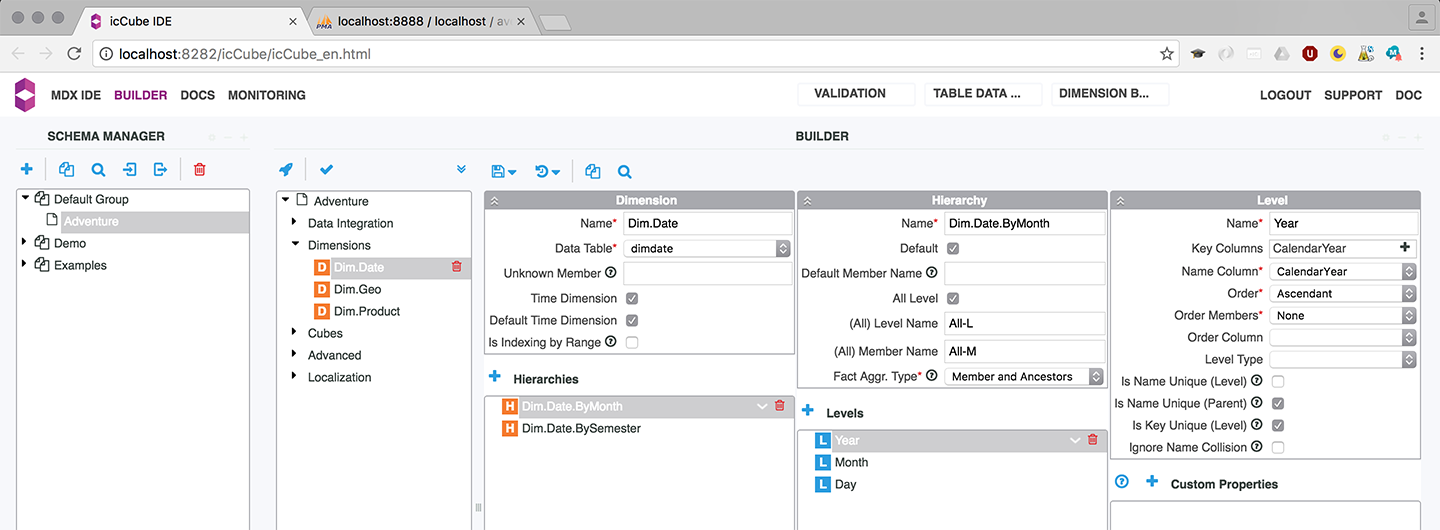
\includegraphics[width=1\linewidth, fbox]{img/dateMonthYear.png}
    \caption{Configuration Dim.Date.ByMonth - Year}
    \label{dateMonthYear}
\end{figure}

\begin{figure}[H]
    \centering
    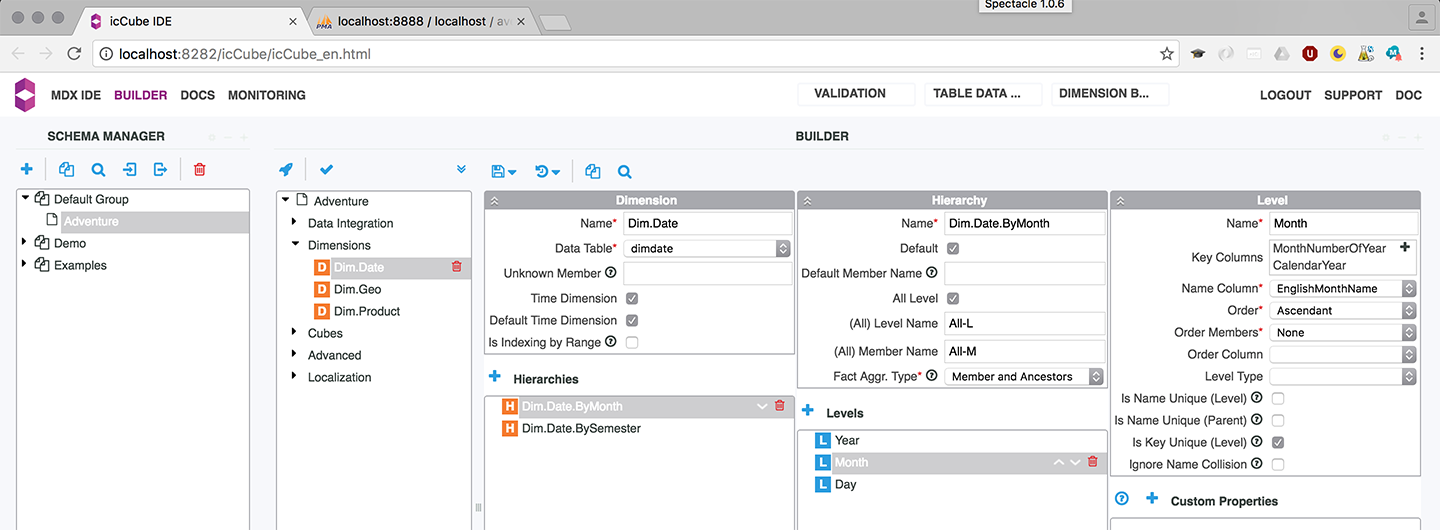
\includegraphics[width=1\linewidth, fbox]{img/dateMonthMonth.png}
    \caption{Configuration Dim.Date.ByMonth - Month}
    \label{dateMonthMonth}
\end{figure}

\begin{figure}[H]
    \centering
    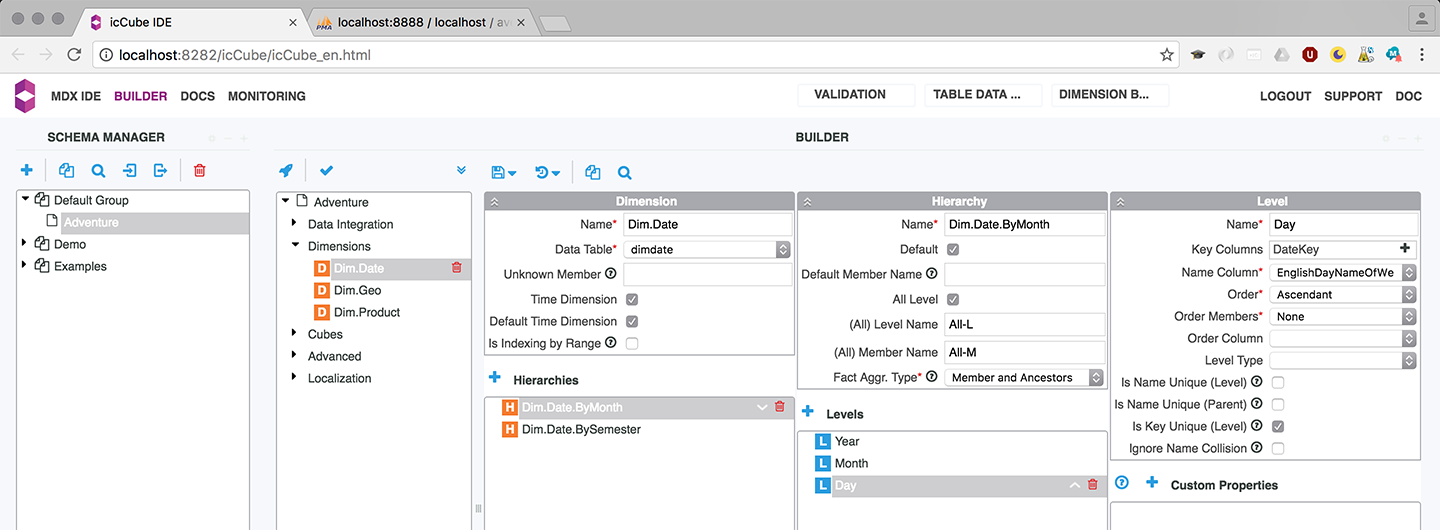
\includegraphics[width=1\linewidth, fbox]{img/dateMonthDay.png}
    \caption{Configuration Dim.Date.ByMonth - Day}
    \label{dateMonthDay}
\end{figure}

\subsubsection*{Hiérarchie Année - Semestre - Trimestre - Jour}

\begin{figure}[H]
    \centering
    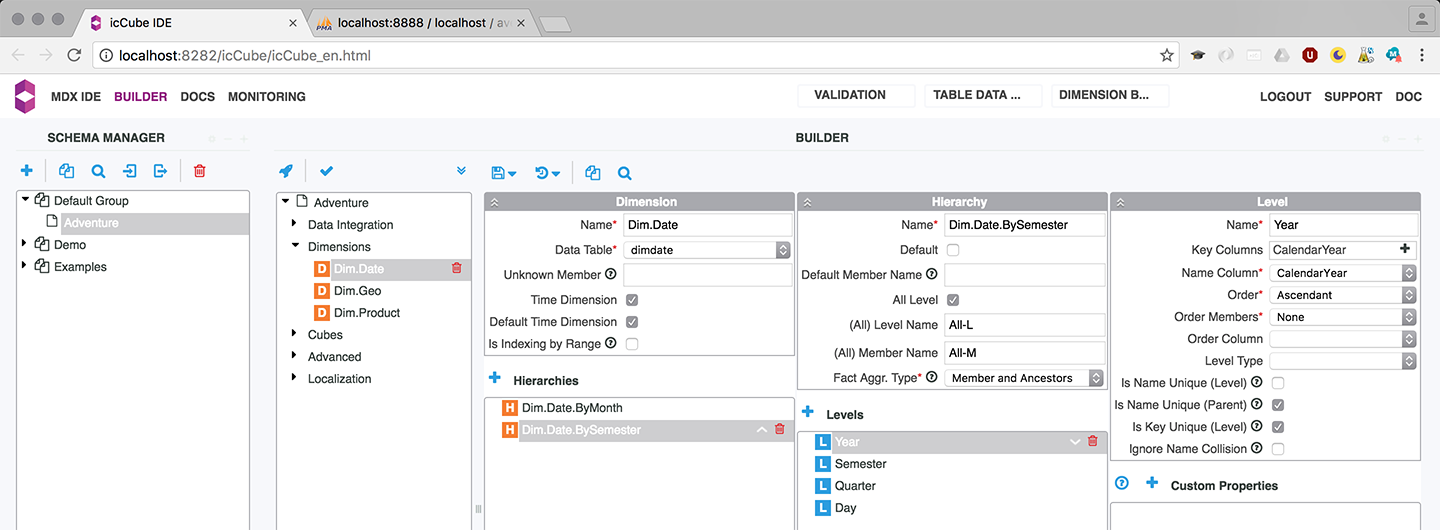
\includegraphics[width=1\linewidth, fbox]{img/dateSemYear.png}
    \caption{Configuration Dim.Date.BySemester - Year}
    \label{dateSemYear}
\end{figure}

\begin{figure}[H]
    \centering
    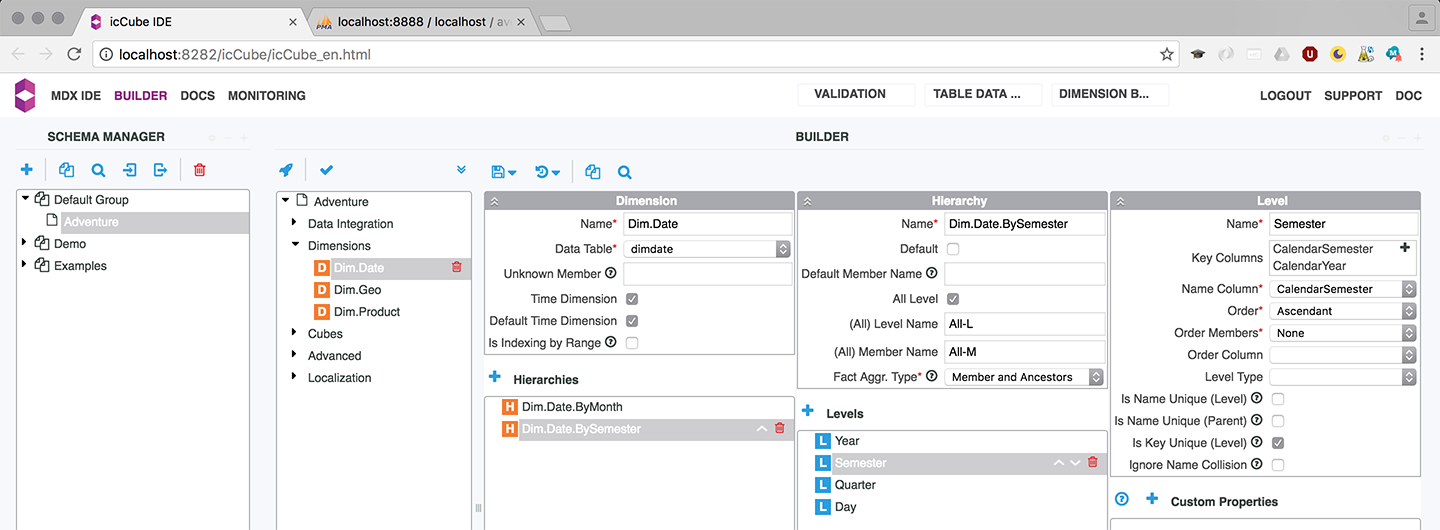
\includegraphics[width=1\linewidth, fbox]{img/dateSemSem.png}
    \caption{Configuration Dim.Date.BySemester - Semester}
    \label{dateSemSem}
\end{figure}

\begin{figure}[H]
    \centering
    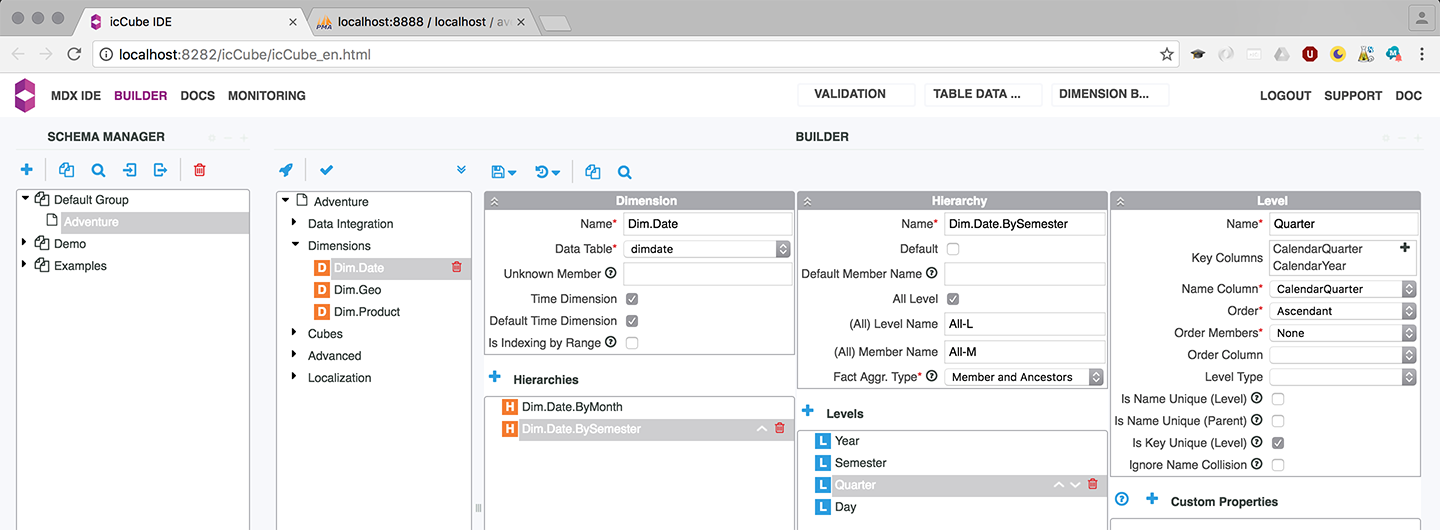
\includegraphics[width=1\linewidth, fbox]{img/dateSemQuarter.png}
    \caption{Configuration Dim.Date.BySemester - Quarter}
    \label{dateSemQuarter}
\end{figure}

\begin{figure}[H]
    \centering
    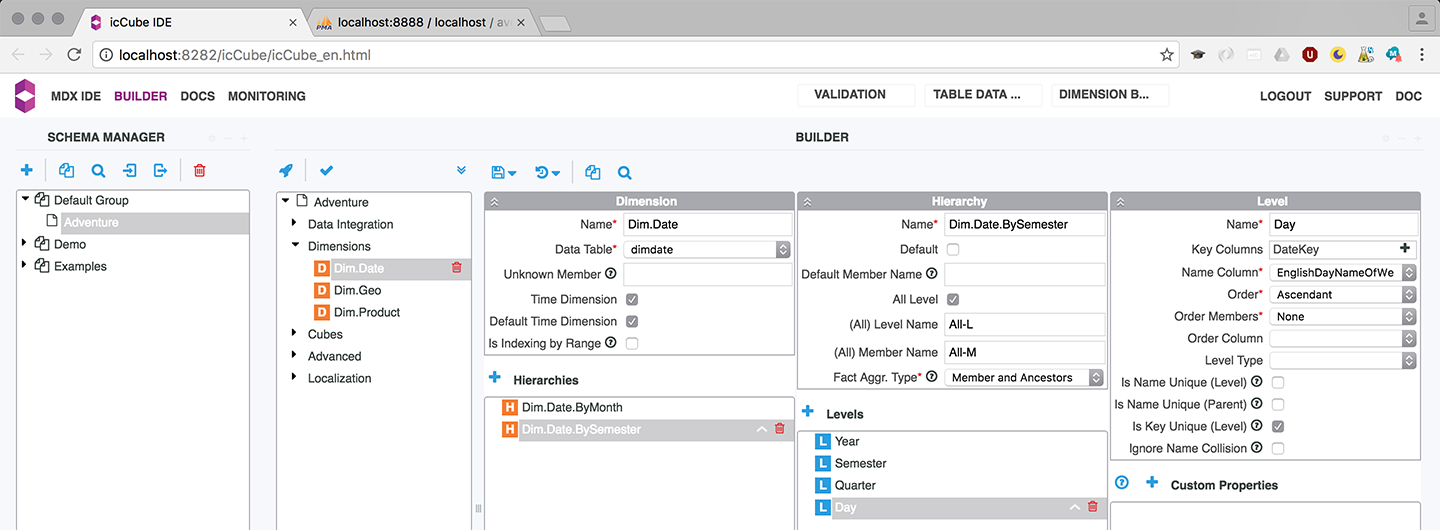
\includegraphics[width=1\linewidth, fbox]{img/dateSemDay.png}
    \caption{Configuration Dim.Date.BySemester - Day}
    \label{dateSemDay}
\end{figure}



\subsection{Dimension des produits}

% Pour la dimension des produits, les informations nécessaires sont réparties dans différentes tables, vous devrez donc utiliser la vue MySql que vous avez créée (point 1). 
% Veuillez aussi mettre des captures d’écran dans votre rapport.

\begin{figure}[H]
    \centering
    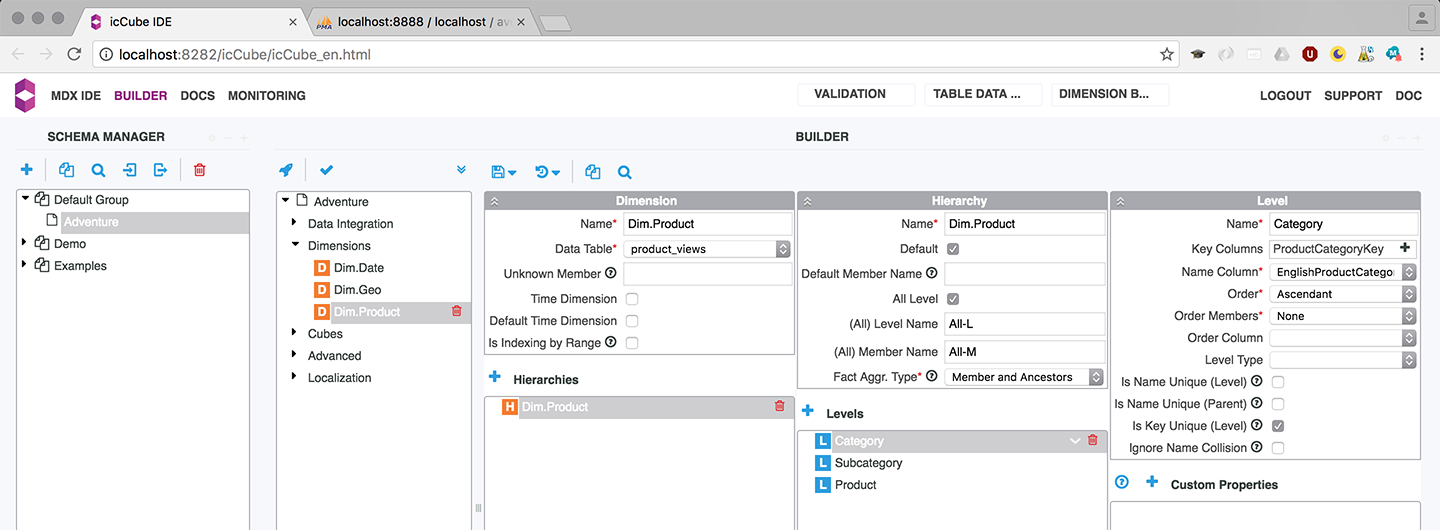
\includegraphics[width=1\linewidth, fbox]{img/prodCat.png}
    \caption{Configuration Dim.Product - Category}
    \label{prodCat}
\end{figure}

\begin{figure}[H]
    \centering
    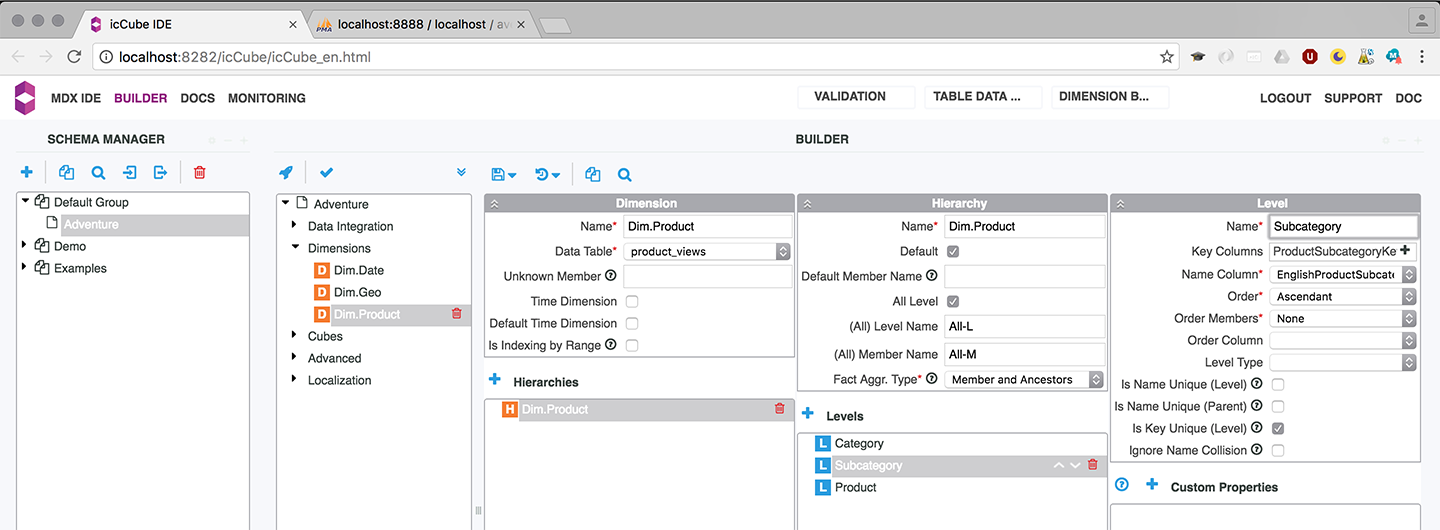
\includegraphics[width=1\linewidth, fbox]{img/prodSubcat.png}
    \caption{Configuration Dim.Product - Subcategory}
    \label{prodSubcat}
\end{figure}

\begin{figure}[H]
    \centering
    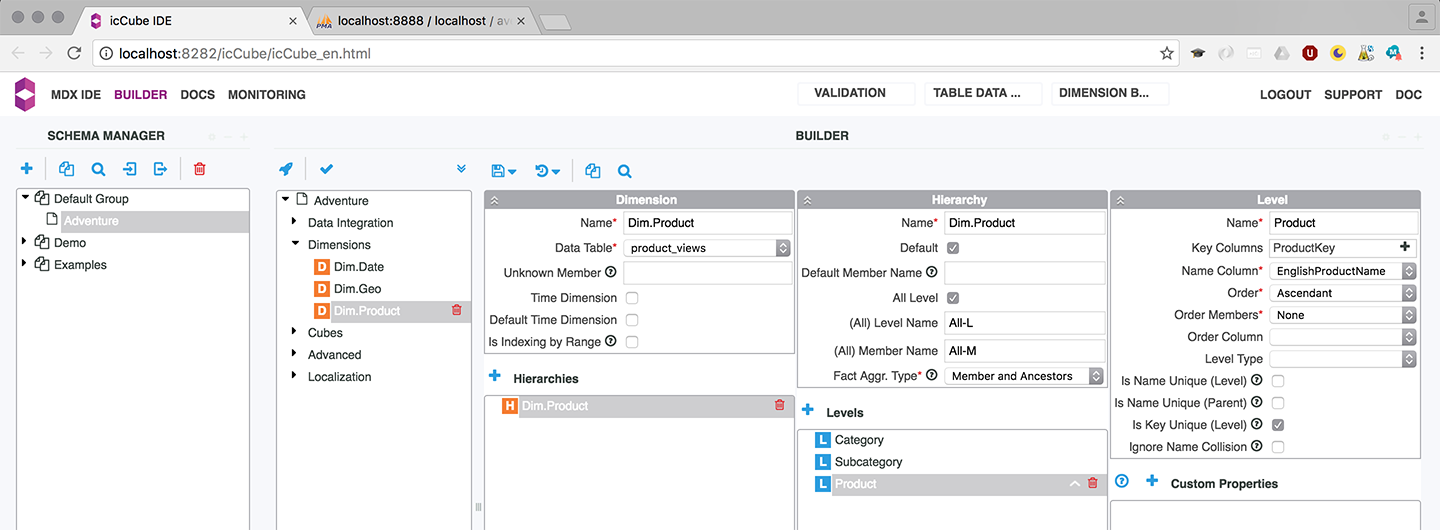
\includegraphics[width=1\linewidth, fbox]{img/prodProd.png}
    \caption{Configuration Dim.Product - Product}
    \label{prodProd}
\end{figure}






\chapter{Exploration}

\section{Slice}

\textbf{Énoncé} : Effectuez une requête simple afin de déterminer le montant total des ventes pour l’année 2008.

\begin{figure}[H]
\centering
\begin{lstlisting}
select [Dim.Date].[Dim.Date.ByMonth].[Year].[2008] on rows,
[Measures].[SalesAmount] on columns from [AdventureCube]
\end{lstlisting}
\caption{Requête Slice : montant total des ventes pour l'année 2008}
\label{lst:reqSlice}
\end{figure}

\begin{figure}[H]
    \centering
    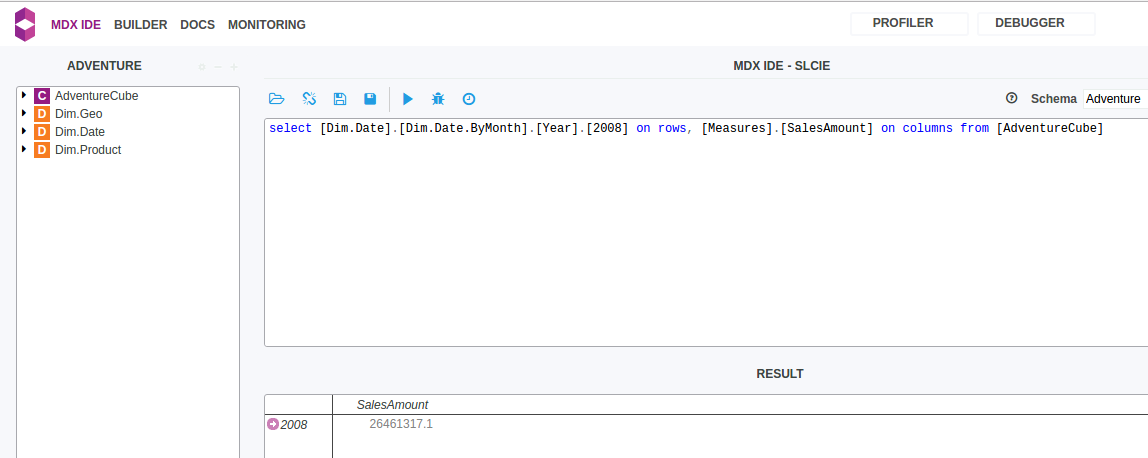
\includegraphics[width=1\linewidth, fbox]{img/requeteSlice.png}
    \caption{Résultat requête Slice : montant total des ventes pour l'année 2008}
    \label{reqSliceResult}
\end{figure}

Le résultat obtenu est : 26461317.1

\section{Dice}

\textbf{Énoncé} : Déterminer le montant des ventes de l’article « Fender Set – Mountain » pour l’année 2008 en Californie. [Accessoires -> Fenders -> Fender Set – Mountain]

\begin{figure}[H]
\centering
\begin{lstlisting}
select [Dim.Date].[Dim.Date.ByMonth].[Year].[2008] on rows,
	   [Measures].[SalesAmount] on columns
from [AdventureCube]
where (
	   [Dim.Geo].[Dim.Geo].[Country].[United States].[California],
	   [Dim.Product].[Dim.Product].[Product].&[485]
      )
\end{lstlisting}
\caption{Requête Dice : montant des ventes de l'article « Fender Set – Mountain » pour l'année 2008}
\label{lst:reqDice}
\end{figure}

\begin{figure}[H]
    \centering
    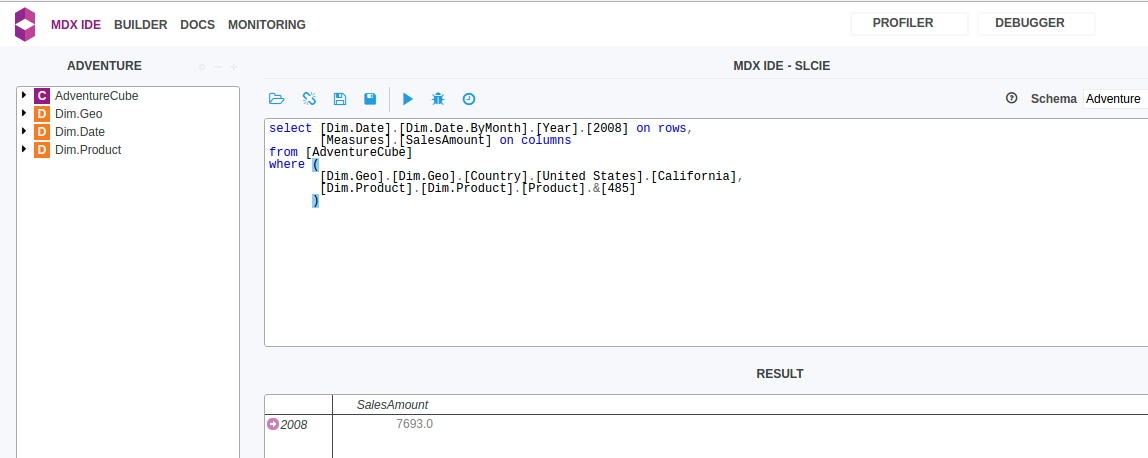
\includegraphics[width=1\linewidth, fbox]{img/requeteDice.png}
    \caption{Résultat requête Dice : montant des ventes de l'article « Fender Set – Mountain » pour l'année 2008}
    \label{reqSliceDice}
\end{figure}

Le résultat obtenu est : 7693

\section{Roll-up}

\textbf{Énoncé} : En utilisant le principe du Roll-up, déterminez le montant des ventes de l’article « Fender Set – Mountain » pour l’ensemble des États-Unis ainsi que pour l’ensemble des pays, toujours pour l’année 2008.

\subsubsection*{Étas-Unis}

\begin{figure}[H]
\centering
\begin{lstlisting}
select ([Dim.Geo].[Country].[United States], [Dim.Product].[Product].&[485]) on columns,
[Measures].[SalesAmount] on rows
from [AdventureCube]
where [Dim.Date].[Dim.Date.ByMonth].[Year].[2008]
\end{lstlisting}
\caption{Requête Roll-up : montant des ventes de l'article « Fender Set – Mountain » Étas-Unis en 2008}
\label{lst:reqRollUpUS}
\end{figure}

\begin{figure}[H]
    \centering
    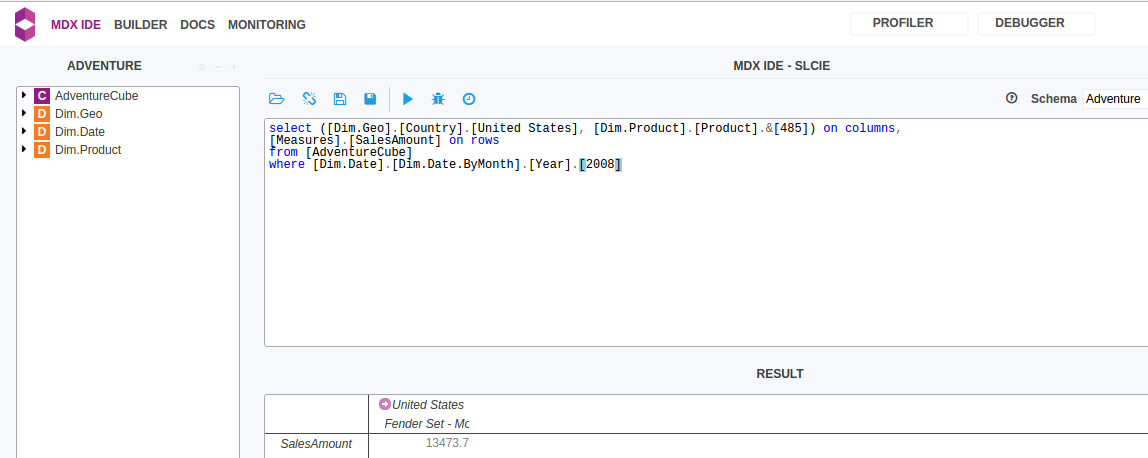
\includegraphics[width=1\linewidth, fbox]{img/requeteRollUpUS.png}
    \caption{Résultat requête Roll-up : montant des ventes de l'article « Fender Set – Mountain » Étas-Unis en 2008}
    \label{reqRollUpResultUS}
\end{figure}

Le résultat obtenu pour les Étas-Unis est : 13473.7

\subsubsection*{Tous les pays}

\begin{figure}[H]
\centering
\begin{lstlisting}
select ([Dim.Geo].[Dim.Geo],[Dim.Product].[Dim.Product].[Product].&[485]) on columns,
[Measures].[SalesAmount] on rows
from [AdventureCube]
where [Dim.Date].[Dim.Date.ByMonth].[Year].[2008]
\end{lstlisting}
\caption{Requête Roll-up : montant des ventes de l'article « Fender Set – Mountain » Étas-Unis en 2008}
\label{lst:reqRollUpUS}
\end{figure}

\begin{figure}[H]
    \centering
    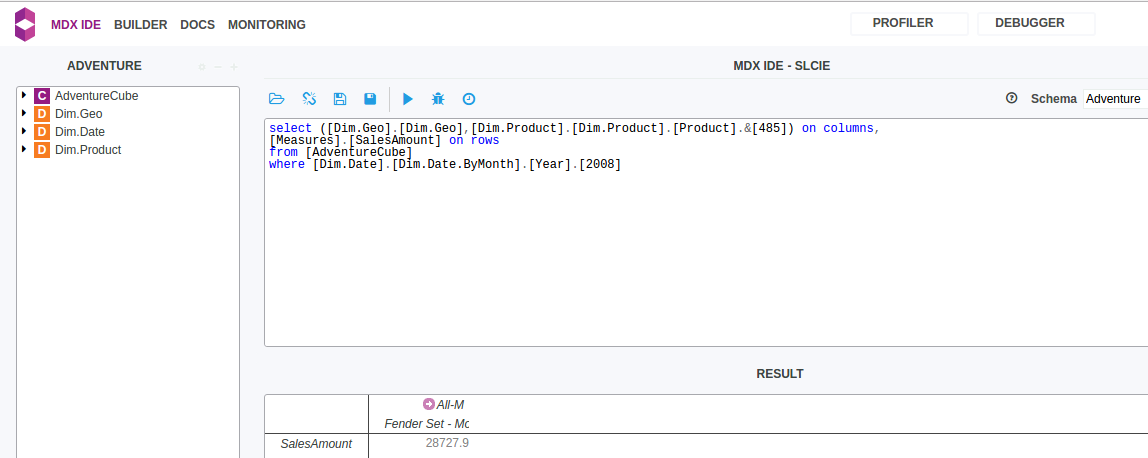
\includegraphics[width=1\linewidth, fbox]{img/requeteRollUpPays.png}
    \caption{Résultat requête Roll-up : montant des ventes de l'article « Fender Set – Mountain » Tous les pays en 2008}
    \label{reqRollUpResultPays}
\end{figure}

Le résultat obtenu pour tous les pays est : 28727.9

\section{Drill-down}

\textbf{Énoncé} : Pour l’ensemble des pays, déterminez quel trimestre de 2008 a été le plus fructueux au niveau des ventes de l’article « Fender Set – Mountain ». Quel a été le montant total des ventes ?

\subsubsection*{Ordre chronologique}

\begin{figure}[H]
\centering
\begin{lstlisting}
select ([Dim.Geo], [Dim.Product].[Product].&[485]) on rows,
[Dim.Date].[Dim.Date.BySemester].[Quarter] on columns
from [AdventureCube]
where [Dim.Date].[Dim.Date.ByMonth].[Year].[2008]
\end{lstlisting}
\caption{Requête Drill-Down - Chronologique}
\label{lst:reqDrill1}
\end{figure}

\begin{figure}[H]
    \centering
    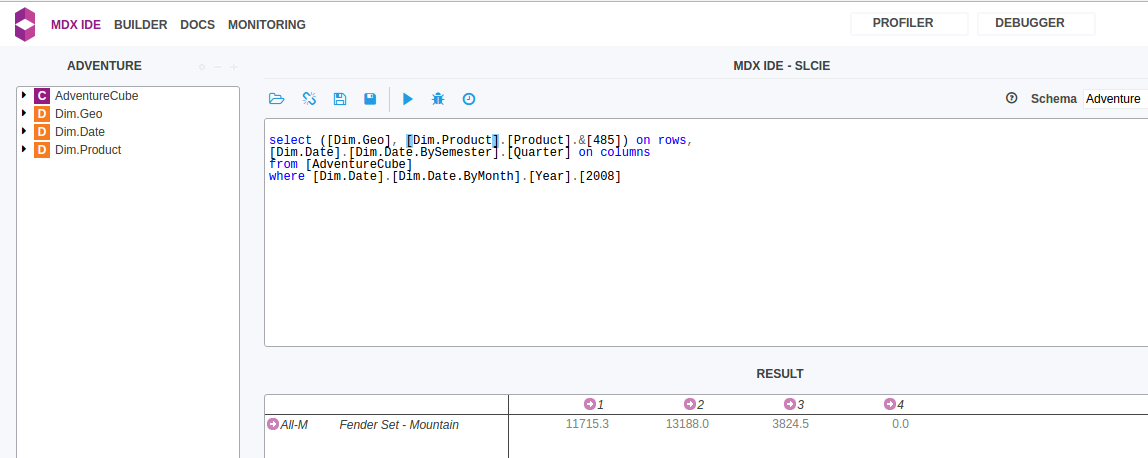
\includegraphics[width=1\linewidth, fbox]{img/requeteDrill1.png}
    \caption{Résultat requête Drill-Down - Chronologique}
    \label{reqDrill1}
\end{figure}

\subsubsection*{Ordre par trimestre le plus fructueux}

\begin{figure}[H]
\centering
\begin{lstlisting}
select ([Dim.Geo], [Dim.Product].[Product].&[485]) on rows,
order([Dim.Date].[Dim.Date.BySemester].[Quarter], [Measures].[SalesAmount], DESC) on columns
from [AdventureCube]
where [Dim.Date].[Dim.Date.ByMonth].[Year].[2008]
\end{lstlisting}
\caption{Requête Drill-Down - Trimestre le plus fructueux}
\label{lst:reqDrill2}
\end{figure}

\begin{figure}[H]
    \centering
    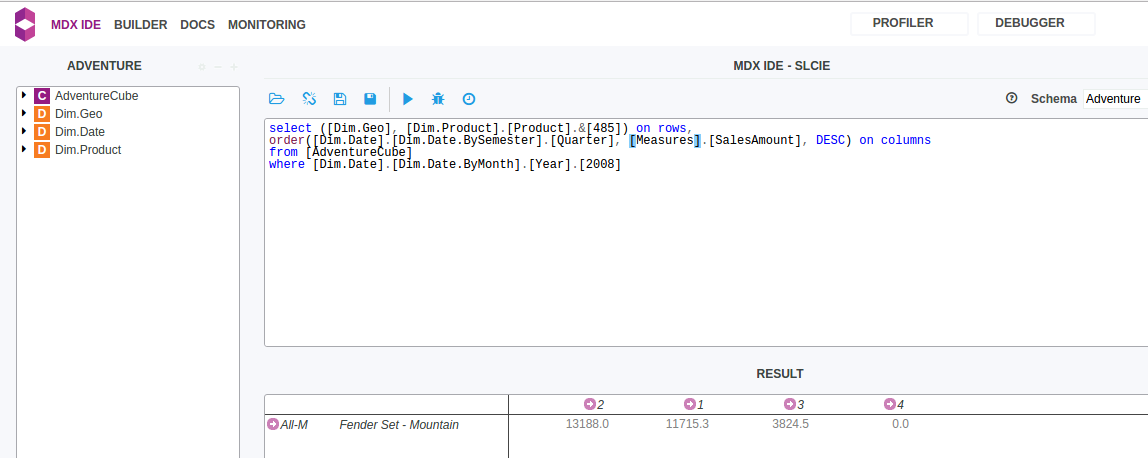
\includegraphics[width=1\linewidth, fbox]{img/requeteDrill2.png}
    \caption{Résultat requête Drill-Down - Trimestre le plus fructueux}
    \label{reqDrill2}
\end{figure}

\chapter{Conclusion}

%TODO 



%	TAIL: Bibliography, Appendix, etc.
%-------------------------------------------------------------------------------
%\appendix

\chapter{Code source}

\section{Wikipedia Ranking}
%\scalafile{code/WikipediaRanking.scala}
\lstinputlisting{code/WikipediaRanking.scala}

\clearpage

\section{DatastoreWrite}
%\javafile{code/DatastoreWrite.java}
\lstinputlisting{code/DatastoreWrite.java}

\clearpage
\backmatter
%\cleardoublepage
\phantomsection
\bibliographystyle{plainnat}
\bibliography{tail/bibliography}
\addcontentsline{toc}{chapter}{Bibliography}


% Add your glossary here
% Add your index here
% Photographic credits (list of pictures&images that have been used with names of the person holding the copyright for them)

\end{document}
